\documentclass[conference]{IEEEtran}
\usepackage{times}

% numbers option provides compact numerical references in the text.
\usepackage[numbers]{natbib}
\usepackage{multicol}
\usepackage[bookmarks=true]{hyperref}

\usepackage{graphicx}

\pdfinfo{
   /Author (Homer Simpson)
   /Title  (Robots: Our new overlords)
   /CreationDate (D:20101201120000)
   /Subject (Robots)
   /Keywords (Robots;Overlords)
}

\begin{document}

% paper title
\title{The Design and Construction of a Novel Variable-Geometry Snake-like Input Device}

% You will get a Paper-ID when submitting a pdf file to the conference system
\author{Author Names Omitted for Anonymous Review. Paper-ID [add your ID here]}



\maketitle

\begin{abstract}
  Humans are skillful.
  By building a bio-inspired manipulable snake-like controller that can be
  molded into a wide variety of shapes, we allow a human controller to telepresently
  specify complex shapes and shape changes.
  We constructed a tetrahelix consisting of seven tetrahedron made of
  adjustable-length members connected via 3D printed Song-Kwon-Kim joints which
  allow manual changes to the shape of the controller. These changes in length are
  digitized and organized via an Arduino and transmitted to more power computers
  where they may specify a shape to be animated or control a robot of similar shape,
  or simply specify relative positions in Cartesian space. Although this research is basic,
  we hope it will eventually amplify human control of in vivo mechanical devices such as
  endoscopes, search-and-rescue robots weaseling into tight spaces, or general purpose
  tetrobots used for planetary space exploration as suggested by
  Prof. Sanderson and his students 20 years ago.
\end{abstract}

\IEEEpeerreviewmaketitle


\section{Introduction}

The possibility of building a robot based on tetrahedra constructed of
tensegrities has been well researched \citet{TetrobotBook,NTRT,paul2006,chen2017soft}.
It is possible to construct a variable geometry truss out of actuators
using tetrahedra as a repeated module that might be expected to have
an advantageous strength-to-weight ratio \citet{mikulas1985sequentially,mirletz2014}.
The existence of the Boerdijk-Coxeter tetrahelix\citet{coxeter1985simplicial}
has long been recognized \citet{fuller1982synergetics,graytetrahelix} as a
geometric means of composing tetrahedra into long beam, which
might combine the structural advanatages of a tetrahedral tensegrity with
snake-like robot motion \citet{hirose1993biologically,liljebäck2012snake}.

By utilizing a 3D-printed jointing system
 which
 supports angular displacement of multiple members coming to central point
 extending previously patented work \citet{song2003spherical} and small-scale
 actuators and microcontrollers, the authors have constructed a relatively
 inexpensive tetrobot. Although some headway has been made in numerical
 control, this papers explores the fundamental idea of using a simulacrum
 controller. A controller which is isomporphic to the robot (but smaller)
 is constructed
 which can be manipulated by hand by an operated. The larger robots mimics
 the motion of the controller. This controller, called the {\em tetrocon},
 has been used to develop a better hexapodal walking and turning gaits
 than previously possible for the tetrobot. Striking an object in space
 with the end effector is easy with the controller. The controller even allows, with some effort,
 locomotion around or over obstacles.  This paper reports on the tetrocon
 and its usage.

 Although developed to control the tetrobot, the controller could be used
 independently as a shape-input device. For example, it could control
 a tentacle animation or, more importantly, a surgical robot that had
 basically snake-like or
 tentacle-like properties, such as an advanced endoscope or arthroscope.

 \section{Design and Manufacture}

 All hardware and software the designs of the controller are free-libre
 open source \citet{anonymous}.

 A tensegrity is a device in which each member only supports and has to
 support either tensile or compressive loads, or both.
 No member has to resist angular displacement.
 Tensegrities usually use cables for the tensile compoments and rods
 for the compessive components. Tensegritie robots vary the length of one or
 the other.
 Since a cable attached to a point can pull in any direction, the tensegrity
 condition is achieved by attaching rods only to cables, not other rods.

 However, \citet{HamlinSandersonCMS} produced a novel concentric
 multilink spherical joint based on parallelograms. Somewhat later
 \citet{song2003spherical} patented a modification of a ball-and-socket
 joint which is rougly similar. 3D printing makes the construction of
 Song-Kwon-Kim joint practical and inexpensive, though it is not necssarily
 superior.

 Such joints allow multiple rods to be connected with spherical rotation
 around a single point, automatically forming a tensegrity.
 If those rods can change length on their own power, they form a
 machine or robot. If those rods can be changed by external forces,
 the form an input device.
 If you build both, you can have robot which mimics a simularcum or
 puppet controller you can shape with your hands.

 \subsection{The Controller}

 The tetrocon device uses 3D printed Song-Kwon-Kim joints. The holes in
 the locking shell of this joint are centered so as to mimic a tetrahelix
 (slightly different configuration would be needed for other configurations.)
 So long as the ratio of maximum to minimum displacement of a member does not
 exceed the golden ratio ($\frac{\sqrt{5} + 1}/2$), the joint does moves
 freely and does not break.

 Linear potentiometers serve as linear dispacement sensors.
 These sensors are held in snap-together 3D printed sleeves, which have
 female parts to receive our universal jointing system. The entire
 system is modular, in the sense that every joint and
 every member is precisely the same.
 It snaps apart easily but is easy to repair.

 Electronically, each of six potentiometers (forming a two-tetrahedra
 modular extention) is connected to a multiplexer, which controllers
 which signal is sent to an Arduino Uno microcontroller. This allows
 the 24 displacment sensors in a 7-tetrahedron controller to be
 digitized. A simple program returns all values upon request in
 JSON.

 A Python program implements a webserver, which allows other software
 to query the state of the 24 channels in the controller simply by
 making a web request.







\begin{figure}
  \centering
  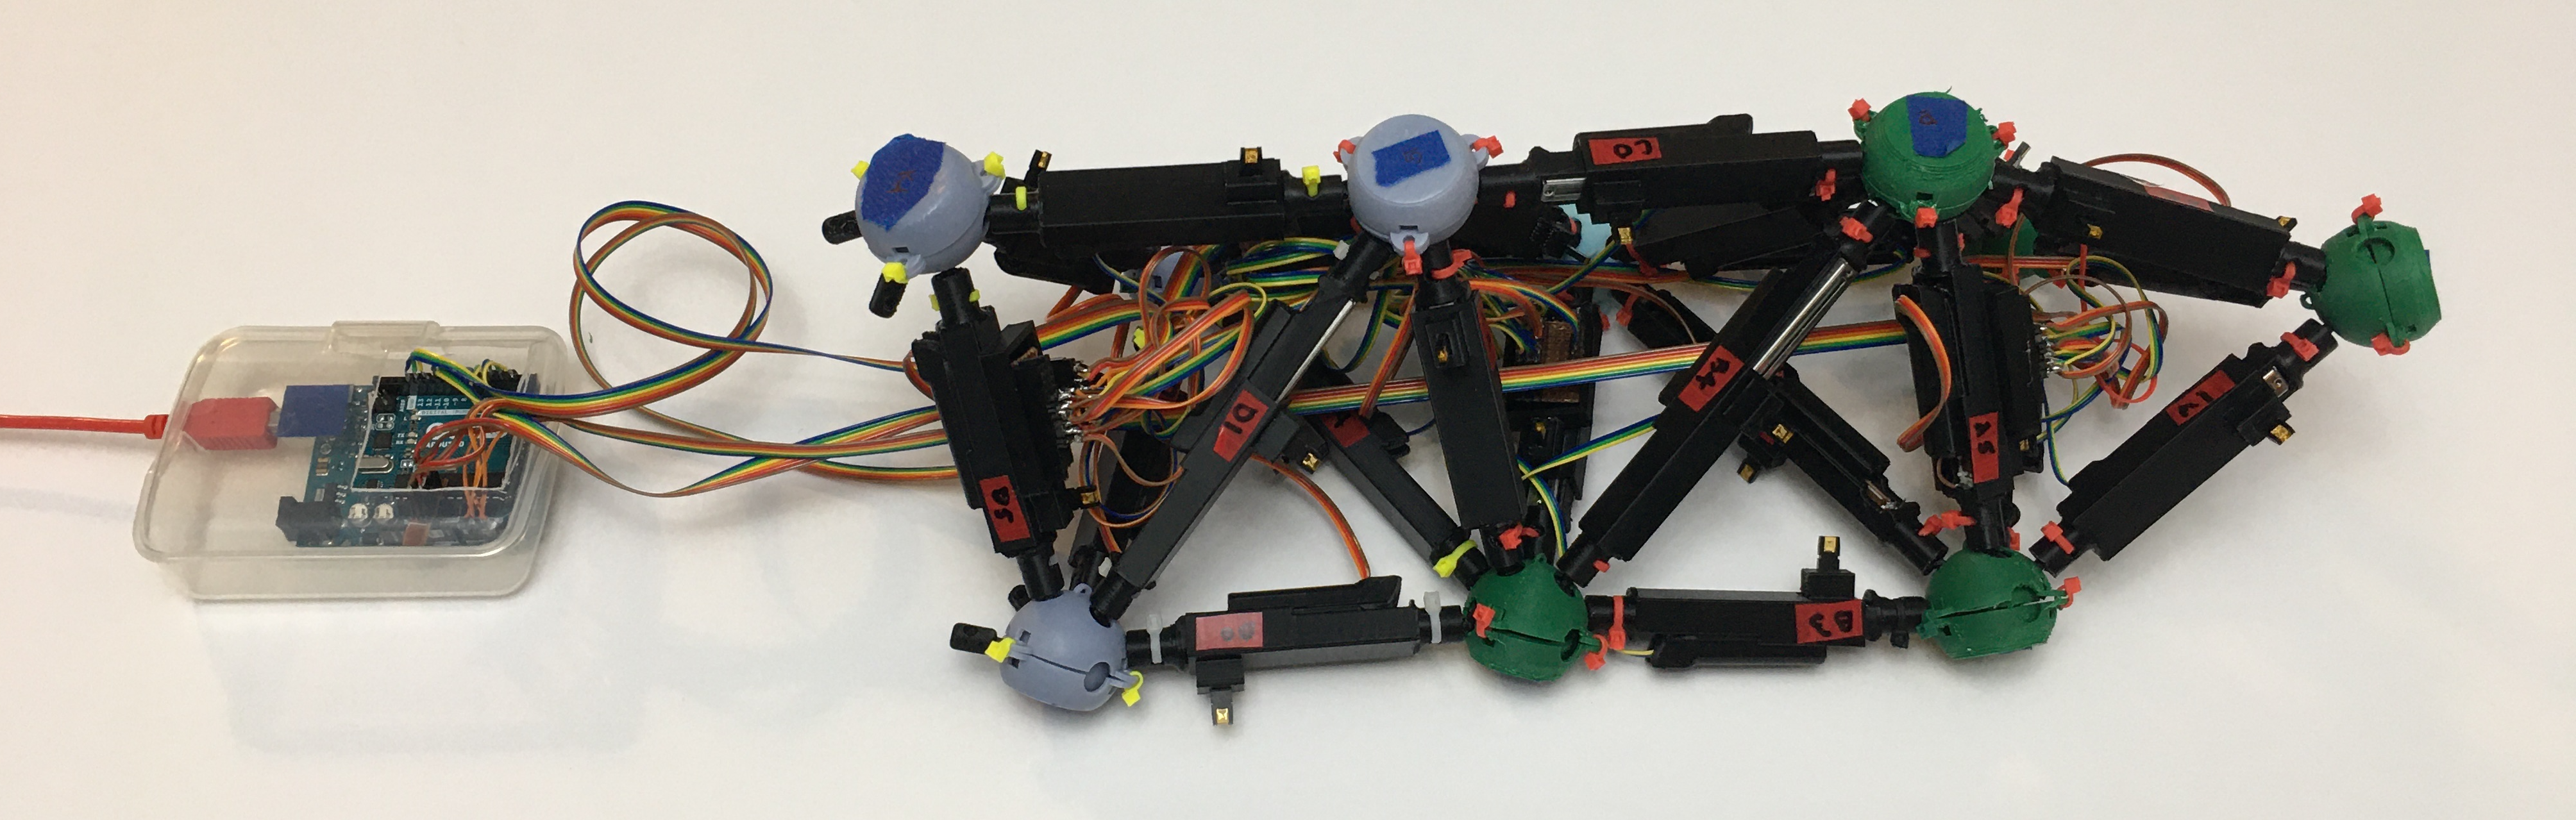
\includegraphics[width=0.5\textwidth]{figures/7TetControllerCropped.png}
    \caption[A 7-tetrahedron Controller]{A 7-tetrahedron Controller}
      \label{fig:7tetcontroller}
\end{figure}

\begin{figure}
  \centering
  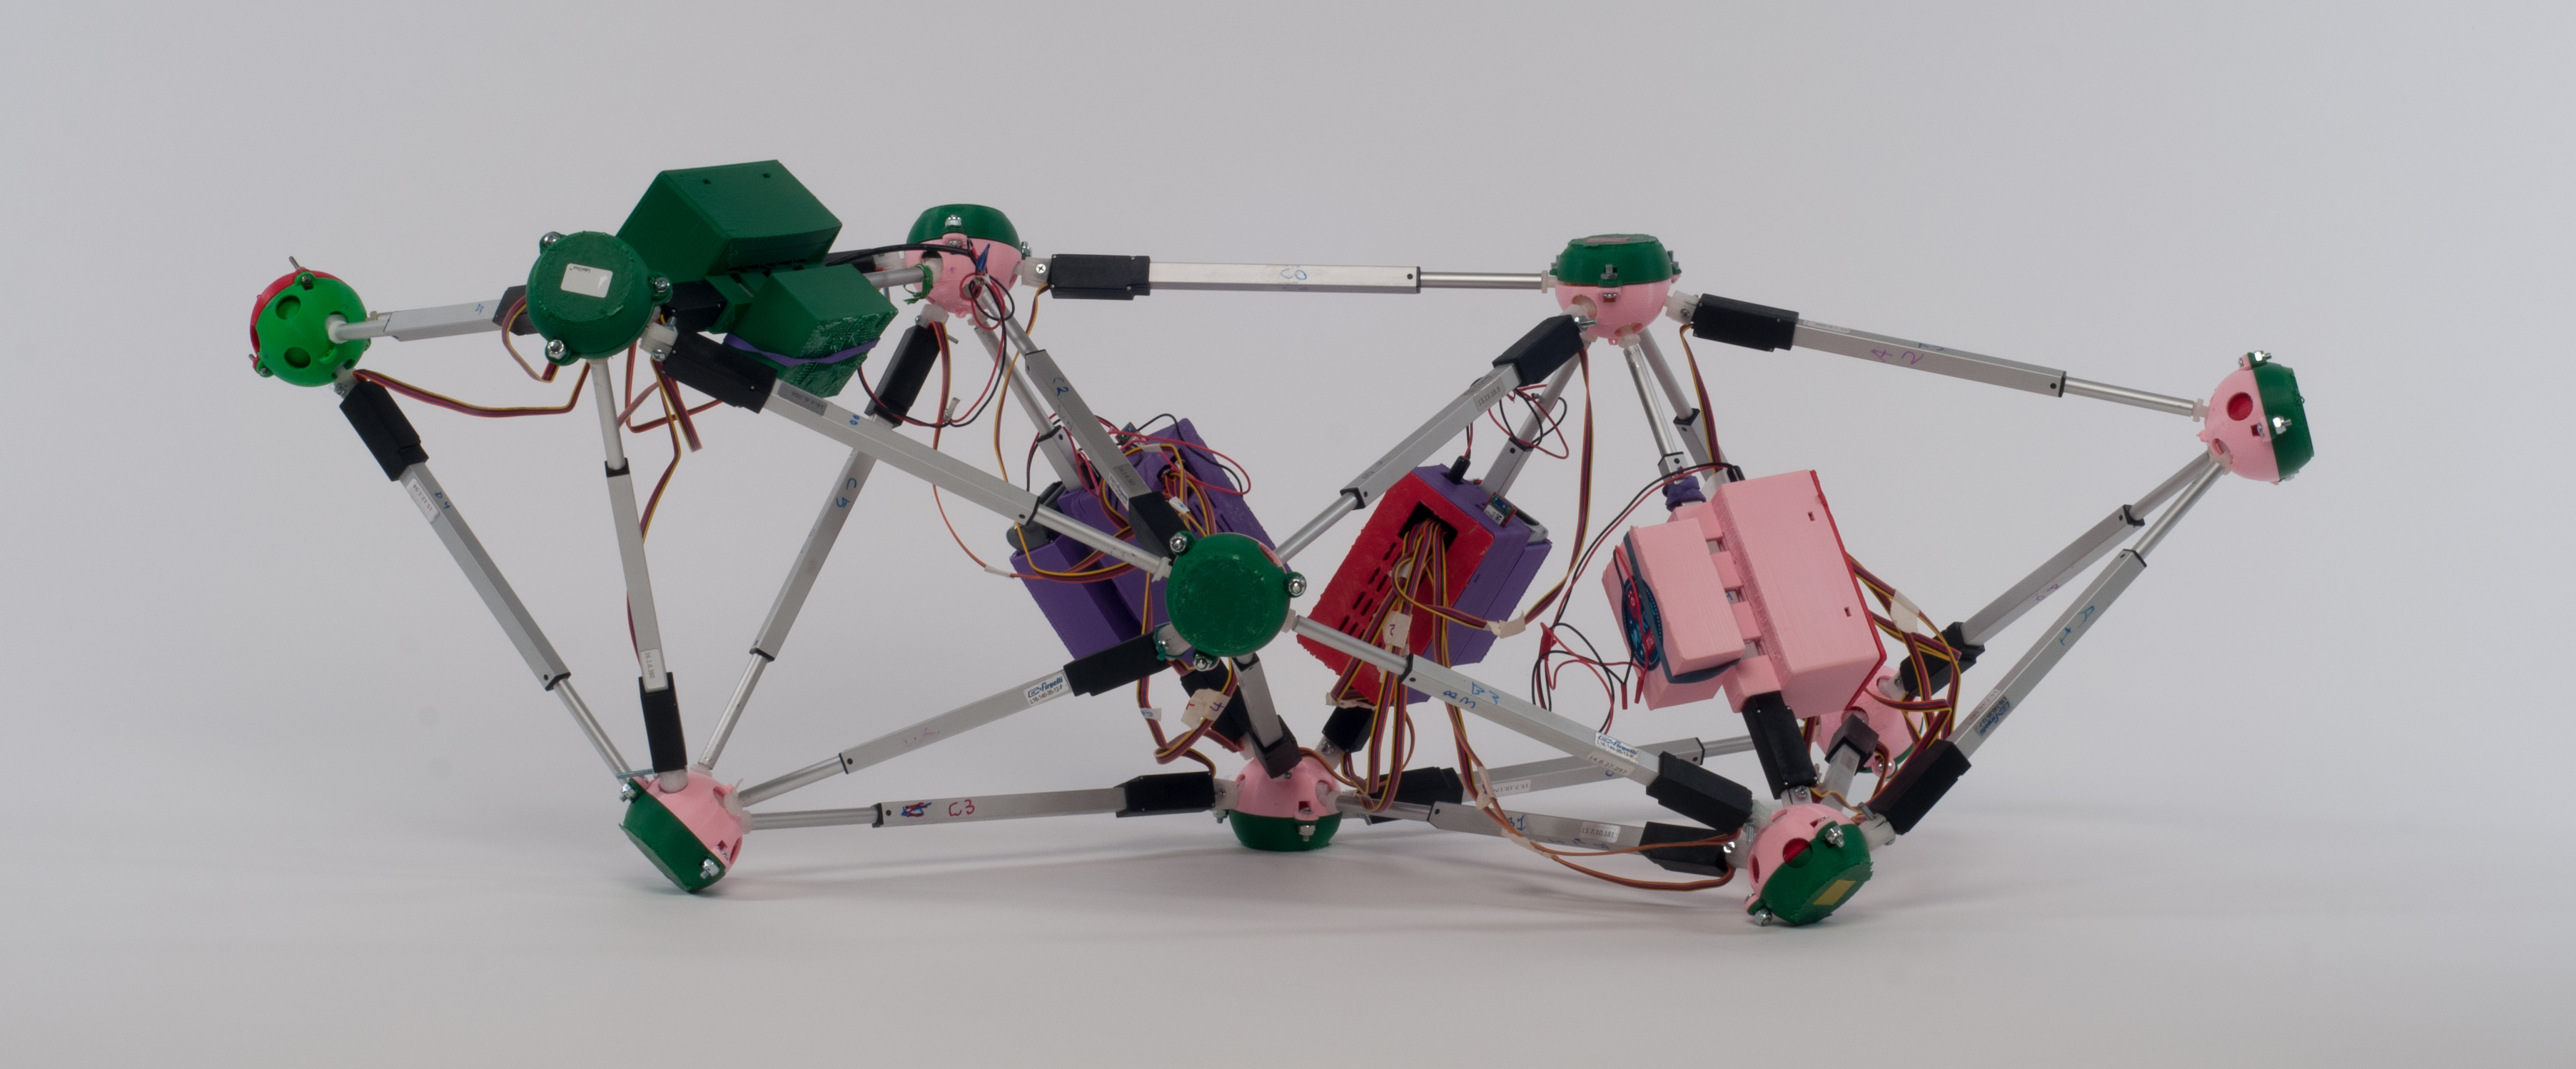
\includegraphics[width=0.5\textwidth]{figures/MedCantedCropped.png}
    \caption[A 7-tetrahedron Robot]{A 7-tetrahedron Tetrobot}
      \label{fig:7tetrobot}
\end{figure}



\section{Conclusion}
\label{sec:conclusion}

The conclusion goes here.

\section*{Acknowledgments}

Some people will be thanked after the anonymous review period.

%% Use plainnat to work nicely with natbib.

\bibliographystyle{plainnat}
\bibliography{references}

\end{document}






%\author{\authorblockN{Michael Shell}
%\authorblockA{School of Electrical and\\Computer Engineering\\
%Georgia Institute of Technology\\
%Atlanta, Georgia 30332--0250\\
%Email: mshell@ece.gatech.edu}
%\and
%\authorblockN{Homer Simpson}
%\authorblockA{Twentieth Century Fox\\
%Springfield, USA\\
%Email: homer@thesimpsons.com}
%\and
%\authorblockN{James Kirk\\ and Montgomery Scott}
%\authorblockA{Starfleet Academy\\
%San Francisco, California 96678-2391\\
%Telephone: (800) 555--1212\\
%Fax: (888) 555--1212}}


% avoiding spaces at the end of the author lines is not a problem with
% conference papers because we don't use \thanks or \IEEEmembership


% for over three affiliations, or if they all won't fit within the width
% of the page, use this alternative format:
%
%\author{\authorblockN{Michael Shell\authorrefmark{1},
%Homer Simpson\authorrefmark{2},
%James Kirk\authorrefmark{3},
%Montgomery Scott\authorrefmark{3} and
%Eldon Tyrell\authorrefmark{4}}
%\authorblockA{\authorrefmark{1}School of Electrical and Computer Engineering\\
%Georgia Institute of Technology,
%Atlanta, Georgia 30332--0250\\ Email: mshell@ece.gatech.edu}
%\authorblockA{\authorrefmark{2}Twentieth Century Fox, Springfield, USA\\
%Email: homer@thesimpsons.com}
%\authorblockA{\authorrefmark{3}Starfleet Academy, San Francisco, California 96678-2391\\
%Telephone: (800) 555--1212, Fax: (888) 555--1212}
%\authorblockA{\authorrefmark{4}Tyrell Inc., 123 Replicant Street, Los Angeles, California 90210--4321}}

\section{RSS citations}

Please make sure to include \verb!natbib.sty! and to use the
\verb!plainnat.bst! bibliography style. \verb!natbib! provides additional
citation commands, most usefully \verb!\citet!. For example, rather than the
awkward construction

{\small
\begin{verbatim}
\cite{kalman1960new} demonstrated...
\end{verbatim}
}

\noindent
rendered as ``\cite{kalman1960new} demonstrated...,''
or the
inconvenient

{\small
\begin{verbatim}
Kalman \cite{kalman1960new}
demonstrated...
\end{verbatim}
}

\noindent
rendered as
``Kalman \cite{kalman1960new} demonstrated...'',
one can
write

{\small
\begin{verbatim}
\citet{kalman1960new} demonstrated...
\end{verbatim}
}
\noindent
which renders as ``\citet{kalman1960new} demonstrated...'' and is
both easy to write and much easier to read.

\subsection{RSS Hyperlinks}

This year, we would like to use the ability of PDF viewers to interpret
hyperlinks, specifically to allow each reference in the bibliography to be a
link to an online version of the reference.
As an example, if you were to cite ``Passive Dynamic Walking''
\cite{McGeer01041990}, the entry in the bibtex would read:

{\small
\begin{verbatim}
@article{McGeer01041990,
  author = {McGeer, Tad},
  title = {\href{http://ijr.sagepub.com/content/9/2/62.abstract}{Passive Dynamic Walking}},
  volume = {9},
  number = {2},
  pages = {62-82},
  year = {1990},
  doi = {10.1177/027836499000900206},
  URL = {http://ijr.sagepub.com/content/9/2/62.abstract},
  eprint = {http://ijr.sagepub.com/content/9/2/62.full.pdf+html},
  journal = {The International Journal of Robotics Research}
}
\end{verbatim}
}
\noindent
and the entry in the compiled PDF would look like:

\def\tmplabel#1{[#1]}

\begin{enumerate}
\item[\tmplabel{1}] Tad McGeer. \href{http://ijr.sagepub.com/content/9/2/62.abstract}{Passive Dynamic
Walking}. {\em The International Journal of Robotics Research}, 9(2):62--82,
1990.
\end{enumerate}
%
where the title of the article is a link that takes you to the article on IJRR's website.


Linking cited articles will not always be possible, especially for
older articles. There are also often several versions of papers
online: authors are free to decide what to use as the link destination
yet we strongly encourage to link to archival or publisher sites
(such as IEEE Xplore or Sage Journals).  We encourage all authors to use this feature to
the extent possible.
